\documentclass[11pt,a4paper]{article}
\usepackage[utf8x]{inputenc}
\usepackage[T1]{fontenc}
%\usepackage{gentium}
\usepackage{mathptmx} % Use Times Font

\usepackage{graphicx} % Required for including pictures
\usepackage{hyperref} % Format links for pdf
\usepackage[british]{babel} % Multilingual bibliographies
\usepackage{natbib}
\setlength{\bibsep}{0.0pt}

\frenchspacing % No double spacing between sentences
\usepackage[margin=1in]{geometry}

\usepackage[all]{nowidow} % Tries to remove widows
\usepackage[protrusion=true,expansion=true]{microtype} % Improves typography, load after fontpackage is selected

\usepackage{lipsum} % Used for inserting dummy 'Lorem ipsum' text into the template

\usepackage[autostyle]{csquotes} % Adds support for single quotes
\usepackage{amsmath}  % Import alignment facilities
\usepackage{subcaption}  % Import alignment facilities
\usepackage{booktabs}

\newcommand{\ra}[1]{\renewcommand{\arraystretch}{#1}}

\title{Popularity of Munros}
\author{Filip Balucha, Advaith Sai Maddipatla, Tudor Finaru}
%\usepackage{natbib}

\begin{document}

\maketitle

%% INSTRUCTIONS:
%%
%% 1. Please rename this file fds-project-option-1.tex,
%% fds-project-option-2.tex, or fds-project-option-3.tex, depending on
%% which project option you are doing. When you submit, please submit
%% the PDF file with the corresponding name.
%% 
%% 2. You can edit either using:
%%
%%    a. Overleaf professional, a collabaratorive LaTeX editor. See
%%       https://www.overleaf.com/edu/edinburgh for documentation. Create an
%%       empty document, and copy the files in this directory to it.
%%
%%    b. A LaTeX editor on your PC - you can commit changes to this
%%       repository to collaborate.
%% 
%% 3. Please keep the section and paragraph headings as they are.
%%
%% 4. The word limit for the Overview section is mandatory. For the
%% other sections word limits are suggested.
%%
%% 5. The page limits must be strictkly adhered to, and depend on if
%% you are working individually, in pairs or in threes:
%%
%%   - Individual: 6 pages 
%%   - Pairs: 8 pages 
%%   - Threes: 10 pages 
%%

% TODO: rename this file!!! absolutely crucial!
\section{Overview}
% 250 words maximum
This paper answers a few key questions regarding Munro hiking by applying statistical methods on data that is freely available online. It aims to explore the reasons behind the popularity of specific hills, and then provides an appropriate clustering of Munros according to their features. In order to achieve this, we use techniques such as linear regression, principal component analysis, and K-Means clustering. The results from these techniques yield good results, enabling us to reach a number of solid conclusions. First of all, we have established the existence of a statistically significant relationship between Munro altitude and number of ascents. Furthermore, we have managed to identify several other factors that have an influence on Munro popularity – for example the numbers of neighbouring Munros, hotels, and the distance to the nearest city. Finally, we have divided the Munros into four well-defined clusters according to their features.

\section{Introduction}
% Suggested 400 words

\paragraph{Context and motivation}

We aim to shed light on the patterns of human behaviour and preferences surrounding Munro hiking – an increasingly popular pastime \cite{CSM}. Many of these hills hold an almost sacred spot in the Scottish psyche, with some locals attaching their very identities to these pieces of timeless, rugged landscape \cite{HAE}. Considering the extensive data on Munros that is available online – as well as the lack of previous scientific literature on the subject – we deemed this topic worthy of further investigation.

\paragraph{Previous work}

There has not yet been a comprehensive study to investigate the patterns that we are trying to observe in this paper. However, there are certainly examples of similar studies carried out about other mountain ranges – a particularly thorough one has been conducted on the Italian Dolomites \cite{HitA}. Among other things, the way the authors 'nested' peaks according to their features has been a useful source of inspiration for our own clustering and linear regression models. 

\paragraph{Objectives}

We are setting out to answer the following questions:
\begin{itemize}
    \item Is there a statistically significant relationship between Munro height and the number of ascents?
    \item What other factors have a significant impact on Munro popularity?
    \item Can Munros be clustered according to their features?
\end{itemize}

\newpage
\section{Data}
% Suggested 300 words
\paragraph{Data provenance}
For the purposes of this paper, we used three datasets:
\begin{itemize}
    \item \textbf{WalkHighlands (WH)}, from which we extracted data on the popularity of Munros as well as the accommodation facilities in their vicinity. This data relies on contributions from registered users – they can select and rate the Munros they have climbed. We retrieved the data using web scraping for the main Munro tables and subpages; additionally, we manually copied the number of facilities for each type of accommodation from the relevant subpages. These methods were chosen after a careful assessment of the T\&Cs \cite{WHTC}.
    \item \textbf{The Database of British and Irish Hills (DoBIH)}, from which we extracted geographical data on the Munros. The origins of this data can be traced in a \textquote{series of articles in Marhofn and Relative Matters magazine}, according to the website. The current editorial team consists of Graham Jackson, Chris Crocker, John Barnard, Simon Edwardes, George Gradwell, Jim Bloomer, and Dave Marshall. The T\&Cs of this dataset are quite liberal, as they impose \textquote{no restrictions on use of the data by third parties}, so long as the terms of the Creative Commons license are respected \cite{DoBIHTC}. Retrieving the data was easy, as it only involved downloading a readily available CSV file.
    \item \textbf{Simplemaps Cities Database (SCD)}, from which we extracted data on British cities' location and population. The data comes from the US National Geospatial-Intelligence Agency, and is freely available to use under an MIT license \cite {SCDBT}. Again, retrieving the data only involved downloading a CSV file.
\end{itemize}

All web scraping was performed in accordance with James Densmore's rules for ethical web scraping \cite{EiWS}. As such, we only scraped data where no API was accessible, we always provided a “User Agent” string to make our intentions clear to the site owner – as well as to provide a way to contact us – and we requested data at a reasonable rate of at most 1 request per 10 seconds. Finally, we only saved the data we absolutely needed, and did not pass it off as our own.

\paragraph{Data description} 

After processing the data and joining the resulting tables, we obtained a dataset with 282 records and variables as outlined in Table~\ref{table:1}.

\begin{table}[h!]
    \caption{The variables present in the final dataset.}
    \label{table:1}
    \centering
    \begin{tabular}{l  l  l} 
        \toprule
        Variable & Type & Description  \\ 
        \midrule
        name & string & Name of the Munro \\ 
        altitude & integer & Altitude of the Munro [m] \\
        ascent\_count & integer & Number of ascents by WH users\\
        \hline
        region & string & Region in which the Munro is located \\
        county & string & County in which the Munro is located\\
        island & string & Island on which the Munro is located\\
        latitude, longitude & float & Coordinates of the Munro's peak\\
        \hline
        bb\_count & integer & Number of B\&Bs in the region\\
        hotel\_count & integer & Number of hotels in the region\\
        hostel\_count & integer & Number of hostels in the region\\
        cottage\_count & integer & Number of cottages in the region\\
        camping\_count & integer & Number of camping and glamping sites in the region\\
        \hline
        nearest\_city\_dist & float & Distance to the city closest to the Munro [km]\\
        nearest\_city\_population & integer & Population of the city closest to the Munro\\
        neighbor\_count\_<$r_1$>\_<$r_2$> & integer & Number of neighbouring Munros within $(r_1,r_2]$ km\\
        population\_<$r_1$>\_<$r_2$> & integer & Population within $(r_1,r_2]$ km\\
        \bottomrule
    \end{tabular}
\end{table}
\paragraph{Data processing}
For the DoBIH data, we only chose Munros. We kept only the relevant columns, which were name, altitude, island, county, and its latitude and longitude.

For the SCD data, we first filtered out cities not in the UK. Then, for each Munro, we computed the distance to and population of the nearest city, as well as the distance to the nearest large city. We considered any city with a population of at least 50,000 to be large, since the 10 largest Scottish cities fulfill this criterion. To represent the various distances from which hikers come, we also computed the total population within increasing ranges of distances from the Munro.

We treated the islands of Mull and Skye separately, since neither Portree nor Tobermory, their corresponding largest settlements, are in the database. Considering that Skye is connected to the mainland via a road bridge, we considered the impact of mainland cities on the popularity of Skye Munros. However, since Mull is isolated from the mainland, we simply replaced all city-related values with NaN.

Merging the WH and DoBIH datasets was challenging. First, we created a unique key for each Munro in both tables. The key of choice was a stringified tuple consisting of name and altitude, since only these two fields are available in both datasets. Sadly, they did not always match exactly - some particular cases were so bad that they needed to be handled manually (e.g. the name “Carn Dearg” appears in DoBIH three times). For the remaining data, we performed fuzzy matching on the keys i.e. we matched a key from WH to the closest key in DoBIH based on string edit-distance. We verified the matched key pairs by flagging any pair for which the difference in altitudes was greater than 10m (i.e. greater than $\approx1\%$ of 1018m – the mean Munro altitude) or if the intersection of their names did not match either name. We also ensured that all keys were unique. We then merged the data and removed unnecessary fields such as the aforementioned keys.

After merging, we computed the number of \textquote{neighbours} for each Munro, that is, the number of Munros located within a \textquote{ring} comprising areas located between 0 and 5 km away, and 5 and 20 km away. The former represents Munros that could be reached on foot as part of a single trek, while the latter other Munros that are within driving distance and could be visited during a single trip. We only considered neighbouring Munros located on the same land mass, since we assume that a climber who is to climb multiple Munros in a restricted area will not want to drive to another island to do so (e.g. Skye).

\section{Exploration and  analysis}

This section provides a summary of our data analysis process. It includes key visualisations which helped us reach our conclusions, as well as interpretations of the results on each step of the process. We split it into 3 parts – each of them corresponds to one of the questions that we seek to answer in our paper.

% Suggested 500 words for individual report; proportionately longer
% for group projects).
\subsection{Assessment of the statistical significance of the relationship between Munro height and the number of ascents}

\begin{figure} [h!]
    \centering
    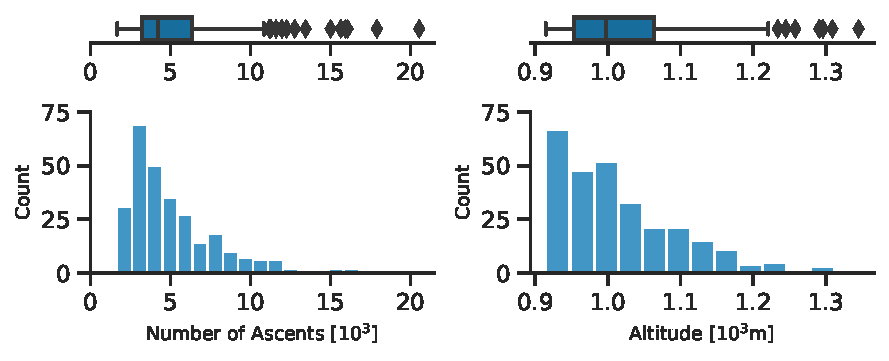
\includegraphics{report/box_dist.pdf}
    \begin{minipage}[t]{.5\linewidth}
        \centering
        \subcaption{The distribution of number of ascents.}
        \label{fds-project-template:fig:box_dist_ascents}
    \end{minipage}%
    \begin{minipage}[t]{.5\linewidth}
        \centering
        \subcaption{The distribution of altitude.}
        \label{fds-project-template:fig:box_dist_altitude}
    \end{minipage}
    \caption{The respective distributions of number of ascents and altitude.}
      \label{fds-project-template:fig:box_dist}
\end{figure}

To get an initial view of the data, we visualise the distributions of Munro ascent counts and heights (Figure~\ref{fds-project-template:fig:box_dist}). We observe that most Munros have been ascended 2500 to 3000-times. The associated box plot tells us that a munro with ascent count greater than 11,000 is considered an outlier (Figure~\ref{fds-project-template:fig:box_dist_ascents}). We also notice that most Munros have an altitude just below 1,000m, with any Munro higher than 1,230m being an outlier (Figure~\ref{fds-project-template:fig:box_dist_altitude}).

In order to better understand and identify some key outliers, it is worth having a look at the scatterplot of ascent count and altitude shown in Figure~\ref{fds-project-template:fig:scatterplot} (note the different increment on the two axes). It comes as little surprise that the two most popular Munros are Ben Lomond and Ben Nevis. In fact, Ben Lomond takes the top spot despite being less than 1,000 metres high. This could likely be explained by its extraordinary popularity with the people of Glasgow, Scotland's most populous city. It is within easy reach of said city, and is well-known as an accessible spot of natural beauty for Glaswegians. On the other hand, Ben Nevis' significant popularity was expected given its status as the tallest mountain in Britain. Its relatively isolated location in the North-West of Scotland does little to deter plenty of people from all over the UK from attempting the comparatively strenuous hike.
% TODO: comment on the different scale in x and y-axis!!!

\begin{figure} [h!]
  \centering
  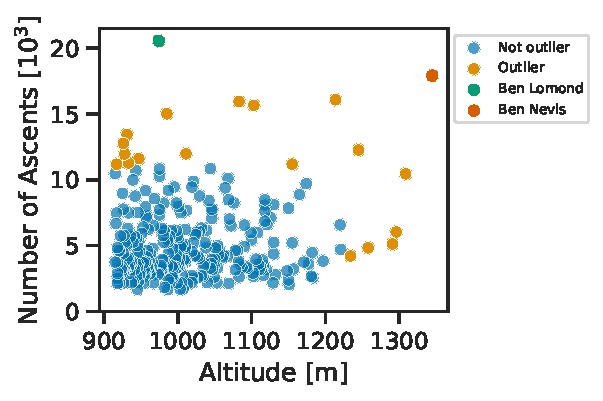
\includegraphics{report/scatterplot.pdf}
  \caption{The scatterplot of ascent count and altitude with key outliers highlighted.}
  \label{fds-project-template:fig:scatterplot}
\end{figure}

We are now in a better position to answer our initial question. Judging by Figure~\ref{fds-project-template:fig:scatterplot}, there appears to be a positive relationship between Munro altitude and ascent count. Moreover, the outliers (e.g. Ben Nevis) should also contribute to that relationship. To formally explore the relationship, we apply Ordinary Least Squares (OLS) linear regression. Consider the linear model: 
$$y=\beta_0 + \beta_1 x$$
where $x$ is altitude and $y$ is ascent count. To evaluate the statistical significance of the relationship, we define the associated null and alternate hypotheses as follows:
\begin{align*}
    H_0 &= \text{The coefficient of altitude in the linear model is equal to zero, i.e. $\beta_1=0$}\\
    H_\text{a} &= \text{The coefficient of altitude in the linear model is not equal to zero, i.e. $\beta_1\neq0$}
\end{align*}

Before applying linear regression, we make sure that the dependent variable is not highly skewed. Its distribution exhibits a right skew (Figure~\ref{fds-project-template:fig:box_dist_ascents}). The distribution is approximately log-normal because the histogram increases to its mode quite quickly and decreases thereafter. Furthermore, the mode is less than the median. To fix this, we log-transform the dependent variable, which yields a distribution that is less skewed and looks approximately normal (Figure~\ref{fds-project-template:fig:dist_log_ascent_count}).
\begin{figure} [h!]
  \centering
  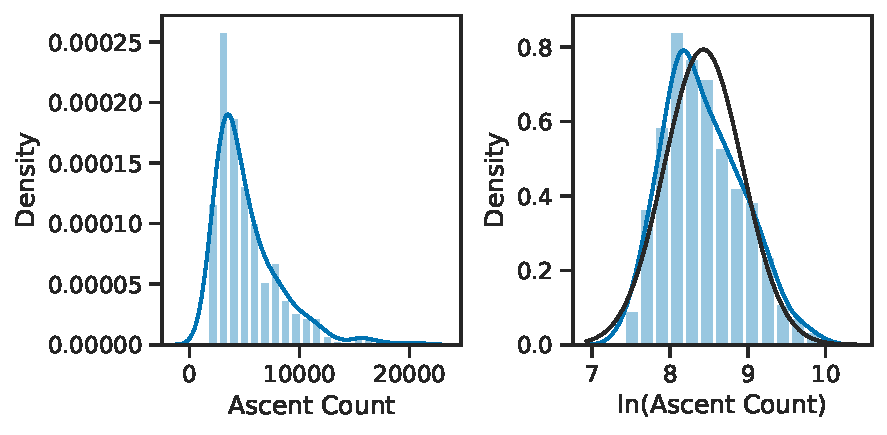
\includegraphics{report/ascent_count_distribution.pdf}
  \caption{The distribution of number of ascents upon log-transformation.}
  \label{fds-project-template:fig:dist_log_ascent_count}
\end{figure}

To aid numerical stability, we normalise the independent variable – i.e. center it around 0. Applying linear regression on the processed data yields a prediction that exhibits a visible increasing trend (Figure~\ref{fds-project-template:fig:q1_prediction}). To diagnose the fit numerically, we use the output of statsmodels.
\begin{figure} [h!]
  \centering
  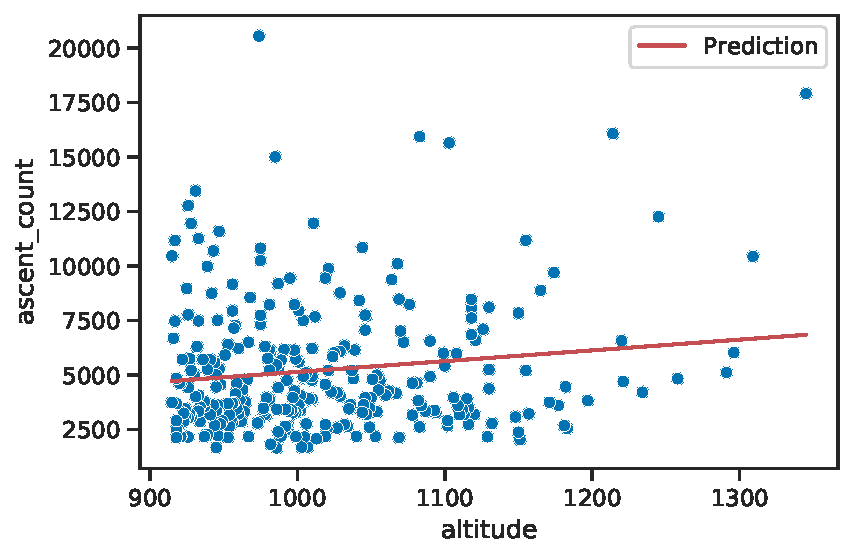
\includegraphics{report/q1_prediction.pdf}
  \caption{The scatterplot of $\ln$(ascent count) against altitude along with fitted values.}
  \label{fds-project-template:fig:q1_prediction}
\end{figure}

The $p$-value of 0.034 for altitude tells us that there is a $\approx 3.4\%$ probability that the relationship between altitude and ascent count may be due to chance. Since $0.034 < 0.05$, we reject the null hypothesis that the coefficient of altitude in the model is 0 at the $5\%$ level. Thus, there is a statistically significant relationship between altitude and ascent count. However, we observe that at $0.016$, the $R^{2}$ value is quite low. This indicates that the model does not predict the data well. This motivates the use of further predictors to aid our analysis.

Since we normalised altitude, it has mean 0. Thus for a Munro of mean altitude, the expected value of $\ln$(ascent count) is given by the intercept $\beta_0=8.4286$. The expected ascent count for a Munro of mean altitude is then $e^{\beta_0}=e^{8.4286}\approx 4576$. 

We now interpret the slope $\beta_1=0.0008$. Let $x$ be the independent variable, and $x^*$ its value upon normalisation, i.e. $x^*=x-\overline{x}$. The regression is of the form $\beta_0 + \beta_1x^* = \ln(y)$ so that $\beta_0 + \beta_1x_1^* = \ln(y_1)$ and $\beta_0 + \beta_1x_2^* = \ln(y_2)$ for two observations. Then
$$\beta_1(x_2 - x_1) = \beta_1\left((x_2 - \overline{x}) - (x_1 - \overline{x})\right) = \beta_1(x_2^* - x_1^*)  = \ln(y_2) - \ln(y_1) = \ln(y_2 / y_1)$$
Consider a unit increase in altitude, such that $x_2-x_1=1$. This gives $e^{\beta_1} = y_2 / y_1$, which can be rewritten as $e^{\beta_1} - 1 = (y_2 - y_1) / y_1$. A unit increase in altitude thus leads to a $100(e^{0.0008} - 1)\% \approx 0.08\%$ increase in altitude. The confidence interval of $[5.57 \times 10^{-5}, 1.00\times10^{-3}]$ tells us that in $95\%$ of all samples that could be drawn, the increase in ascent count will be within $[5.70\times10^{-3}, 1.00\times10^{-1}]\%$.
% TODO y-axis numbering -1.5 to 1.5 on the right
Finally, to validate our approach, we inspect the distribution of residuals (Figure~\ref{fds-project-template:fig:uni_residuals_dist}). They are approximately normally distributed, which is an assumption of linear regression. Furthermore, the variance of residuals does not change as a function of the predicted values of the independent variable (Figure~\ref{fds-project-template:fig:uni_residuals_yhat}). Thus, the dataset is not heteroscedastic. Therefore, linear model was a reasonable choice for the problem at hand.
\begin{figure} [h!]
    \centering
    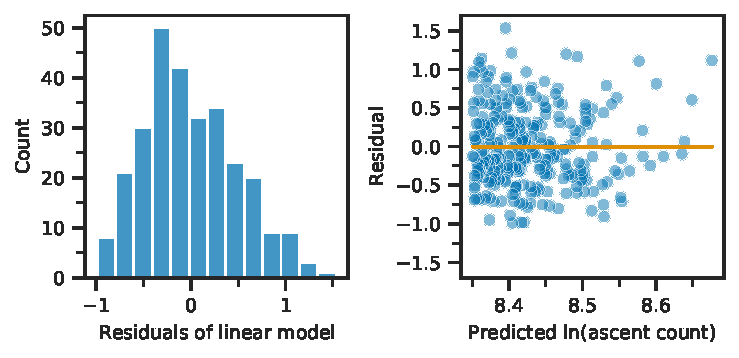
\includegraphics{report/uni_residuals.pdf}
    \begin{minipage}[t]{.5\linewidth}
        \centering
        \subcaption{The distribution of the residuals.}
        \label{fds-project-template:fig:uni_residuals_dist}
    \end{minipage}%
    \begin{minipage}[t]{.5\linewidth}
        \centering
        \subcaption{The scatterplot of residuals against predictions.}
        \label{fds-project-template:fig:uni_residuals_yhat}
    \end{minipage}
    \caption{The residual plots for the univariate linear regression model.}
    \label{fds-project-template:fig:uni_residuals}
\end{figure}

\subsection{Other factors that have a significant impact on Munro popularity}
Moving on to our second question, we need to perform some feature selection on our data. The technique we will be using only expects continuous data, so we ignore categorical or boolean variables. We now standardise the dataset – this helps with numerical stability because some features have a vastly different range of values (e.g. population can be in the thousands, whereas hotel\_count is in the tens).

We use scikit-learn's SelectKBest class to select features. We score the features using the scoring function f\_regression, which is equivalent to running a univariate linear regression test for each independent variable. According to the official documentation \cite{scikit-learn}, f\_regression first computes the Pearson correlation coefficient between the regressor and the target. It outputs a $p$-value, which corresponds to the null hypothesis that there is no linear interaction between between the regressor and the target. We pick the regressors whose $p$-value falls below a certain threshold. As in the previous section, we choose the threshold to be 0.05, such that the null hypothesis can be rejected at the $5\%$ level. That is, we pick only those regressors for which there is a $5\%$ probability that the linear interaction with the target is due to chance.

Before we apply multivariate OLS linear regression, we ensure that there is not significant multicollinearity between our features since that could negatively affect numerical stability, and hence jeopardise the quality of our model. To this end, we inspect the correlation matrix for the selected independent features. All correlation coefficients are below 0.8, and so we do not need to remove any features.

We now apply OLS regression. We will use each of the standardised features as regressors. The target will be the log-transformed ascent count, for the same reason as in previous section. We find that the variables population\_25\_50 and hostel\_count both have quite high $p$-values of over 0.2. This is likely due to multicollinearity with other population- and accommodation-related features, and it is therefore safe to remove these.

After reapplying OLS, we obtain a good fit with an adjusted $R^{2}$ of 0.525. In addition, we notice that all the features in model have a $p$-value of less than 0.01. This indicates the obtained coefficients are reliable.

We now wish to interpret the output of statsmodels. Since the regressors are standardised and the target is log-transformed, we first need to transform them to an interpretable format. We are interested in the impact of a unit change in a regressor on the target. The linear regression is of the form 
$$\beta_0+\beta_1z^{(1)}+ \dots + \beta_n z^{(n)}=\ln(y)$$ 
where $z^{(i)}$ is the standardised $i$-th regressor. To interpret the response in the target to a unit increase in the $i$-regressor, we let $x^j = 0, (\forall j \neq i)$. Then we have $\beta_0 + \beta_i z^{(i)} = \ln(y)$. Now $\beta_i (z_2^{(i)} - z_1^{(i)}) = \ln(y_2) - \ln(y_1)=\ln(y_2/y_1)$. Since 
$z^{(i)} = (x^{(i)} - \overline{x}^{(i)})/\sigma_{x^{(i)}}$
due to standardisation, we may rewrite the above as $\beta_i (x_2^{(i)} - x_1^{(i)})/\sigma_{x^{(i)}} =\ln(y_2/y_1)$. Skipping steps similar to those in previous section, we arrive at $\exp(\beta_i / \sigma_{x^{(i)}}) - 1 = (y_2 - y_1) / y_1$. This result means that a unit increase in an original feature leads to a $100\left(\exp(\beta_i / \sigma_{x^{(i)}}) - 1\right)\%$ increase in ascent count. We now transform the coefficients accordingly; the results can be seen in Table~\ref{table:2}.
% NOTE: \phantom{-} allows us to align negative and positive numbers, please do not remove it
\begin{table} [h!]
\centering
\caption{The values and confidence intervals of transformed coefficients.}
\begin{tabular}{l l l l}
\toprule
    Feature & 
    Response [\%] & 
    Response (CI Lower) [\%] & 
    Response (CI Upper) [\%] \\
\midrule
altitude & $\phantom{-}8.74 \times 10^{-2}$ & $\phantom{-}3.76\times 10^{-2}$ & $\phantom{-}1.37\times 10^{-1}$ \\
hotel\_count & $-7.08\times 10^{-1}$ & $-9.84\times 10^{-1}$ & $-4.32\times 10^{-1}$ \\
neighbor\_count\_5\_20 & $-1.31$ & $-1.81$ & $-8.05\times 10^{-1}$ \\
nearest\_city\_dist & $-5.12\times 10^{-1}$ & $-8.88\times 10^{-1}$ & $-1.35\times 10^{-1}$ \\
pop\_0\_25 & $\phantom{-}2.55 \times 10^{-3}$ & $\phantom{-}1.32\times 10^{-3}$ & $\phantom{-}3.78\times 10^{-3}$ \\
pop\_50\_75 & $\phantom{-}3.27 \times 10^{-5}$ & $\phantom{-}2.42\times 10^{-5}$ &  $\phantom{-}4.11\times 10^{-5}$ \\
pop\_75\_100 & $\phantom{-}3.53 \times 10^{-5}$ & $\phantom{-}2.81\times 10^{-5}$ &  $\phantom{-}4.25\times 10^{-5}$\\
\bottomrule
\label{table:2}
\end{tabular}
\end{table}

The intercept gives the expected value of ascent count on a log scale when all regressors are 0. The intercept is 8.4286 which implies the expected number of ascents is then $e^{8.4286} \approx 4576$ ascents. The most dominant feature is neighbor\_count\_5\_20. Every extra neighbouring Munro within 5-20km reduces the ascent count by $ \approx 1.3\%$. The other dominant features are the number of hotels, wherein each extra hotel reduces ascent count by $\approx 0.71\%$, and the distance to the nearest city, such that each extra kilometer distance leads to a $\approx 0.5\%$ decrease in ascent count. As implied by the first section, altitude also has an impact on ascent count, albeit smaller. Namely, each meter of altitude increases ascent count by $\approx 0.87\%$. There is also a slight positive impact on ascent count associated with population within 0-25km and 50-100km.

% TODO: fix references to figures
We now plot the residuals of our fit against the predictions, as well as the distribution of our errors. As can be seen in Figure~\ref{fds-project-template:fig:multi_residuals_dist}, our errors are normally distributed, which is an assumption of linear regression, and there is no heteroscedasticity exhibited either. This means that using the linear model was a good choice.
\begin{figure} [h!]
    \centering
    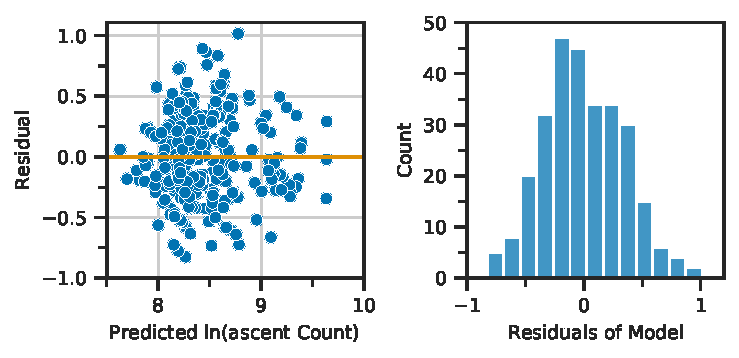
\includegraphics{report/multi_residuals_dist.pdf}
    \begin{minipage}[t]{.5\linewidth}
        \centering
        \subcaption{The distribution of the residuals.}
        \label{fds-project-template:fig:mul_residuals_dist}
    \end{minipage}%
    \begin{minipage}[t]{.5\linewidth}
        \centering
        \subcaption{The scatterplot of residuals against predictions.}
        \label{fds-project-template:fig:mul_residuals_yhat}
    \end{minipage}
    \caption{The residual plots for the multivariate linear regression model.}
    \label{fds-project-template:fig:multi_residuals_dist}
\end{figure}
\subsection{Clustering Munros according to their features}
Moving on to our final question, we aim to cluster Munros according to the independent features. This may help us discover a sub-structure within the dataset and help us understand it better.

Before performing K-Means Clustering, we need to reduce the number of independent variables. This is because as a distance-based method, K-Means suffers from the \textquote{curse of dimensionality} and will perform poorly when applied to a vast dataset. Hence, we perform PCA on the dataset. In order to determine the appropriate number of components to be used, we plot a scree plot to find the knee. It represents the point at which adding more principal components would not explain a significant variance in the data. Figure~\ref{fds-project-template:fig:scree_plot} shows that the first 3 principal components help explain a considerable amount of variance. Using the cumulative plot, we see that this is about $60\%$ of the variance. We thus transform the dataset using the first 3 principal components.
\begin{figure} [h!]
    % TODO: split into a and b!!!
    \centering
    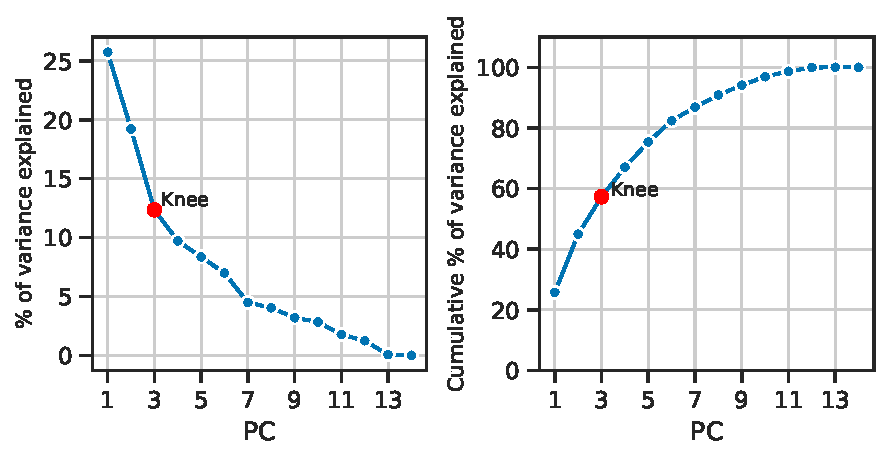
\includegraphics{report/scree_plot.pdf}
    \begin{minipage}[t]{.5\linewidth}
        \centering
        \subcaption{Scree plot.}
        \label{fds-project-template:fig:scree_plot_def}
    \end{minipage}%
    \begin{minipage}[t]{.5\linewidth}
        \centering
        \subcaption{Cumulative scree plot.}
        \label{fds-project-template:fig:scree_plot_cum}
    \end{minipage}
    \caption{Visual diagnostics for PCA.}
    \label{fds-project-template:fig:scree_plot}
\end{figure}
\begin{figure} [h!]
  \centering
  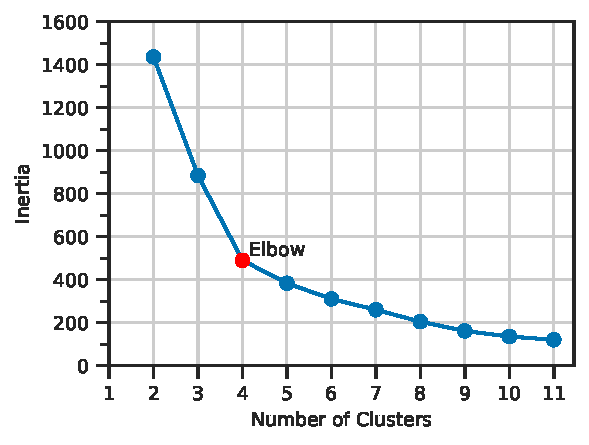
\includegraphics{report/k_screeplot.pdf}
  \caption{K Scree plot}
  \label{fds-project-template:fig:k_screeplot}
\end{figure}
In order to determine the appropriate number of clusters, we inspect the inertia (i.e. the sum of squared errors) of our K-Means model with increasing number of clusters (Figure~\ref{fds-project-template:fig:k_screeplot}). 

To find optimal number of clusters and avoid overfitting, we use the elbow method. As the number of clusters increases, the clusters can explain a greater fraction of variance, reducing inertia. However, there will be a point (the elbow) after which the inertia will decrease significantly \cite{wiki:elbow} – resulting in overfitting. There is a clear elbow at $k = 4$ (Figure~\ref{fds-project-template:fig:k_screeplot}); thus, the optimal number of clusters is 4. We now perform K-Means. Since we cluster in 3 dimensions, we plot the predictions on a 3D plot and indicate the clusters' centroids (Figure~\ref{fds-project-template:fig:3d_clusters}). We now use the information about clusters to inspect the features that contribute to each cluster. To obtain a summary measure for each feature, we compute its for each cluster.

\begin{figure} [h!]
  \centering
  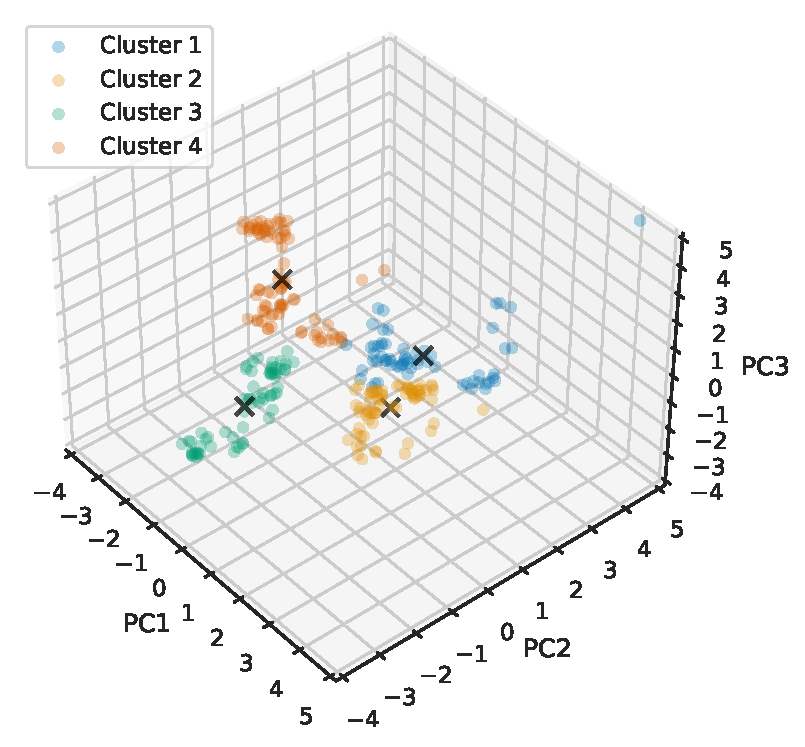
\includegraphics{report/3d_clusters.pdf}
  \caption{3D Clustering of Munros}
  \label{fds-project-template:fig:3d_clusters}
\end{figure}
The average Munro in Cluster 1 has \textasciitilde 2000 inhabitants within 25km, while the nearest city has \textasciitilde 10,000 inhabitants and is \textasciitilde 35km away. This cluster has the largest population 25-100km away out of all clusters. At about 60, it also has the largest number of hotels. It also has a fair amount of bed and breakfast accomodations (about 50). It also has the lowest the number of neighbouring Munros: slightly above 2. Since there are very few neighbouring Munros and there are a lot of (presumably relatively high-end) hotels near these Munros, we expect this cluster to comprise of fairly \textquote{exclusive} Munros which are suitable for visitors from a larger city (which makes them quite popular, too). Two examples of Munros that fall into this category are Ben Lomond and Ben Lawers.

The average Munro in Cluster 2 does not have a large city within 100km. The nearest city is about \textasciitilde 45km away with a population slightly higher than \textasciitilde 7,500. The dominant accommodation type for this cluster are cottages and camping sites, and there are relatively few B&Bs, hotels and hostels. It has about 25 neighboring Munros within 20km. We are therefore dealing with a region with a fairly high number of Munros, with relatively few accommodation facilities and also quite far away from any major cities. Munros that belong to this cluster are fairly isolated and slightly less popular - two examples would be Mount Keen and Ben Hope.

For the average Munro in Cluster 3, the closest city is more than 50km away, but has \textasciitilde 20,000 people – the most across all clusters. It has the largest number of cottages and campings out of all clusters, with relatively fewer B&Bs, hotels and hostels. At more than 4, it also has the largest number of neighboring Munros within 5km. Visitors to Munros included in this cluster might wish to hike several neighboring peaks during their trip and stay at a cottage or camping site. At \textasciitilde 6,000 ascents, these Munros are fairly popular – perhaps some inhabitants of the nearby large city are regular visitors, or the high concentration of nearby Munros makes the entire area a popular hiking destination. The latter point is supported by the inclusion of peaks such as Cairn Gorm and The Cairnwell in this cluster; both of these are located in the Cairngorms Natural Park, one of Scotland's prime areas for hiking.

The average Munro in Cluster 4 has the largest number of people within 25km across all clusters, but relatively few people beyond that. The nearest city is \textasciitilde 25km away and has a population of about 10,000. Other larger settlements lie beyond 75km away. The dominant accommodation types are B&Bs and hostels. At almost 25, it has the largest number of neighboring Munros within 5-20km. Two examples of peaks that belong to this cluster are Ben Nevis and Stob Dearg; these are both located near Fort William and Glencoe in North-West Scotland, an area famous for its high concentration of dramatic Munros – which certainly ensures a large number of neighboring peaks. Apart from a few minor nearby towns that also present a number of accommodation facilities, Munros in this cluster seem to be quite isolated compared to others – and this definitely applies to the two aforementioned examples.

\section{Discussion and conclusions}
% Suggested 400 words.

\paragraph{Summary of findings}
First of all, we have proven that there exists a statistically significant relationship between Munro altitude and number of ascents – taller Munros can generally be expected to exhibit higher ascent counts. We have also explored the influence of other factors on the number of ascents. Some of our results were perhaps surprising – for instance a higher number of neighboring Munros seems to negatively affect ascent count – however most of them were intuitive e.g. Munros located near densely populated areas can be expected to have a higher ascent count. Finally, we have clustered the peaks into four different categories according to their features. We expanded on this by emphasising the correspondence between specific clusters and various moutaineous regions of Scotland.
\paragraph{Evaluation of own work: strengths and limitations}
Our models should be quite reliable – owing to the fact that we only use techniques that fit the given context well. We also aim to be rigorous in our working, providing mathematical justifications to further clarify certain transformations we applied to the data, as well as our plotting choices.

As a result of this, our conclusions should mostly be trustworthy; however, the nature of the data might affect their accuracy somewhat. Perhaps the most important thing to note is that our Munro climbing data is limited to the number of ascents by separate individuals – and we are using this as a proxy for Munro popularity when dealing with Question 2. Additionally, it is worth noting that WalkHighlands requires users to register before allowing them to contribute. This means that the group of people who contributed to the data we are using might not be fully representative of all hikers. The contributors can be expected to be active internet users with a remarkable passion for hiking – which is not necessarily the case for every Munro climber.
\paragraph{Comparison with any other related work}
Scarpa and Thiene have also explored the patterns of human behaviour and preferences surrounding hiking in a certain area – namely the Italian Dolomites \cite{HitA}. Their analysis went slightly deeper than ours, and mostly focused on the manner in which specific mountaineous sites can be substituted for others, provided that some similar features exist between them. There has been no similar study regarding Scottish Munros, and hence our work still stands as a relevant paper, albeit minimal in its scope – and it is certainly worth considering extending it.
\paragraph{Improvements and extensions}
First of all, we could improve our work by considering more factors that lead to Munro popularity; however, this might be limited by the amount of data that is freely available online. Additionally, we could take a similar approach to Scarpa and Thiene, and look for substitution patterns between different Munros – our clustering might prove extremely useful for this \cite{HitA}. Finally, we were considering implementing a Munro recommendation system, through which users would receive Munro climbing suggestions based on their recorded preferences.
\bibliographystyle{unsrt}
\bibliography{fds-project}
\end{document}
